% \documentclass[11pt,a4paper]{article}
\documentclass[11pt,a4paper]{article}
%%%%%%%%%%%%%%%%%%%%%%%%% Credit %%%%%%%%%%%%%%%%%%%%%%%%

% template ini dibuat oleh martin.manullang@if.itera.ac.id untuk dipergunakan oleh seluruh sivitas akademik itera.

%%%%%%%%%%%%%%%%%%%%%%%%% PACKAGE starts HERE %%%%%%%%%%%%%%%%%%%%%%%%
\usepackage{graphicx}
\usepackage{caption}
\captionsetup[table]{name=Tabel}
\captionsetup[figure]{name=Gambar}
\usepackage{tabulary}   
% \usepackage{amsmath}
\usepackage{fancyhdr}
% \usepackage{amssymb}
% \usepackage{amsthm}
\usepackage{placeins}
% \usepackage{amsfonts}
\usepackage{graphicx}
\usepackage[all]{xy}
\usepackage{tikz}
\usepackage{verbatim}
\usepackage[left=2cm,right=2cm,top=3cm,bottom=2.5cm]{geometry}
\usepackage{hyperref}
\hypersetup{
    colorlinks,
    linkcolor={red!50!black},
    citecolor={blue!50!black},
    urlcolor={blue!80!black}
}
\usepackage{libertine}
\usepackage{libertinust1math}
\usepackage[T1]{fontenc}
\usepackage{inconsolata}

\usepackage{caption}
\usepackage{subcaption}
\usepackage{multirow}
\usepackage{psfrag}
\usepackage[T1]{fontenc}
\usepackage[scaled]{beramono}
% Enable inserting code into the document
\usepackage{listings}
\usepackage{xcolor} 
% custom color & style for listing
\definecolor{codegreen}{rgb}{0,0.6,0}
\definecolor{codegray}{rgb}{0.5,0.5,0.5}
\definecolor{codepurple}{rgb}{0.58,0,0.82}
\definecolor{backcolour}{rgb}{0.95,0.95,0.92}
\lstdefinestyle{mystyle}{
	backgroundcolor=\color{backcolour},   
	commentstyle=\color{green},
	keywordstyle=\color{codegreen},
	numberstyle=\tiny\color{codegray},
	stringstyle=\color{codepurple},
	basicstyle=\ttfamily\footnotesize,
	breakatwhitespace=false,         
	breaklines=true,                 
	captionpos=b,                    
	keepspaces=true,                 
	numbers=left,                    
	numbersep=5pt,                  
	showspaces=false,                
	showstringspaces=false,
	showtabs=false,                  
	tabsize=2
}
\lstset{style=mystyle}
\renewcommand{\lstlistingname}{Kode}
%%%%%%%%%%%%%%%%%%%%%%%%% PACKAGE ends HERE %%%%%%%%%%%%%%%%%%%%%%%%


%%%%%%%%%%%%%%%%%%%%%%%%% Data Diri %%%%%%%%%%%%%%%%%%%%%%%%
\newcommand{\stuid}{120140116}
\newcommand{\student}{\textbf{Muhammad Qomarudin (\stuid{})}}
\newcommand{\course}{\textbf{Sistem Operasi (IF2223)}}
\newcommand{\assignment}{\textbf{01}} % tugas ke...

%%%%%%%%%%%%%%%%%%% using theorem style %%%%%%%%%%%%%%%%%%%%
\newtheorem{thm}{Theorem}
\newtheorem{lem}[thm]{Lemma}
\newtheorem{defn}[thm]{Definition}
\newtheorem{exa}[thm]{Example}
\newtheorem{rem}[thm]{Remark}
\newtheorem{coro}[thm]{Corollary}
\newtheorem{quest}{Question}[section]
%%%%%%%%%%%%%%%%%%%%%%%%%%%%%%%%%%%%%%%%
\usepackage{lipsum}%% a garbage package you don't need except to create examples.
\usepackage{fancyhdr}
\usepackage[ddmmyyyy]{datetime}
\pagestyle{fancy}
\lhead{ \student }
\rhead{ \thepage}
\cfoot{\textbf{HandsOn 1 : Working With Linux}} % ini untuk judul tugas
\renewcommand{\headrulewidth}{0.4pt}
\renewcommand{\footrulewidth}{0.4pt}

%%%%%%%%%%%%%%  Shortcut for usual set of numbers  %%%%%%%%%%%

\newcommand{\N}{\mathbb{N}}
\newcommand{\Z}{\mathbb{Z}}
\newcommand{\Q}{\mathbb{Q}}
\newcommand{\R}{\mathbb{R}}
\newcommand{\C}{\mathbb{C}}
\setlength\headheight{14pt}

%%%%%%%%%%%%%%%%%%%%%%%%%%%%%%%%%%%%%%%%%%%%%%%%%%%%%%%555

\begin{document}
\thispagestyle{empty}
\begin{center}
	
\includegraphics[scale = 0.15]{Figure/ifitera-header.png}
	\vspace{0.1cm}
\end{center}
\noindent
% change font family for header section only
%{\fontfamily{LinuxLibertineT-OsF}\large\selectfont 
{\large
\rule{17cm}{0.2cm}\\[0.3cm]
Nama: \student \hfill Tugas Ke: \assignment\\[0.1cm]
Mata Kuliah: \course \hfill Tanggal: \today\\
\rule{17cm}{0.05cm}
\vspace{0.1cm}
}


%%%%%%%%%%%%%%%%%%%%%%%%%%%%%%%%%%%%%%%%%%%%% BODY DOCUMENT %%%%%%%%%%%%%%%%%%%%%%%%%%%%%%%%%%%%%%%%%%%%%

\section{Tujuan Hand On}
	Hands on ini merupakan bentuk lain dari Praktikum matakuliah Sistem Operasi yang bertujuan untuk
	memeperkenalkan Sitem Operasi Linux kepada mahasiswa.
	Dengan di perkenalkannya Sitem Optrasi linux,
	diharapkan mahasiwa dapat mengenmbngkan pemahamannya dan juga dapet bermanfaat pada saat tertentu juka di butuhkan.

\section{Spesifikasi Sistem}
    Sistem yang digunakan adalah sebuah sistem berbasis Linux versi Ubuntu 20.04 LTS. Untuk Sistem bisa mengunakan Boot langsung, atau mengunakan sitem virtual Mecine. selain sitem itu sendiri dibutuhkan sebuah browser yang terinstall di sitem opreasi linux.
	\begin{figure}[h]
		\centering
		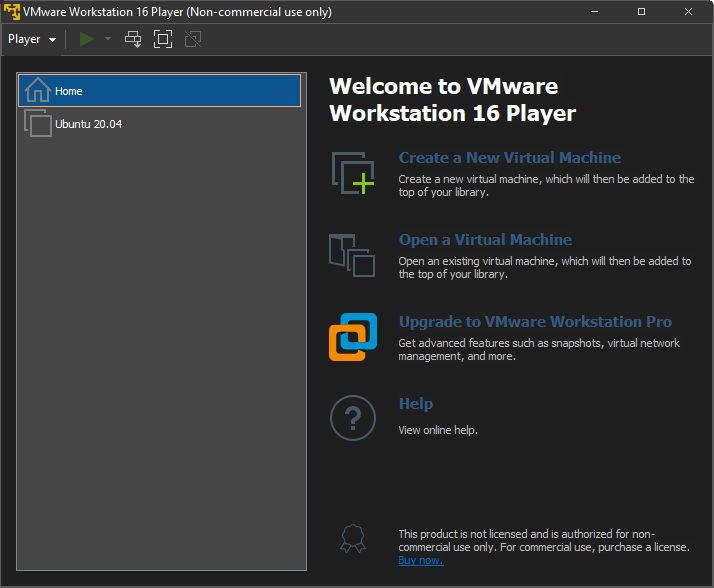
\includegraphics[width=0.8\textwidth]{figure/VM ware.png}
		\caption{boot Ubuntu melalui VM ware}
	\end{figure}
 
\section{Pembahasan Tut 1}
\subsection{Tut 1.1 echo}
    Pada bagian ini, sistem menjalankan perintah \textit{echo}, di mana user mengetikkan "echo Hello World" dan kemudian di exekkusi oleh sistem.
	fungsi \textit{echo} berfungsi untuk mencetak atau menampilakan kata pada layar.
	\begin{figure}[h]
		\centering
		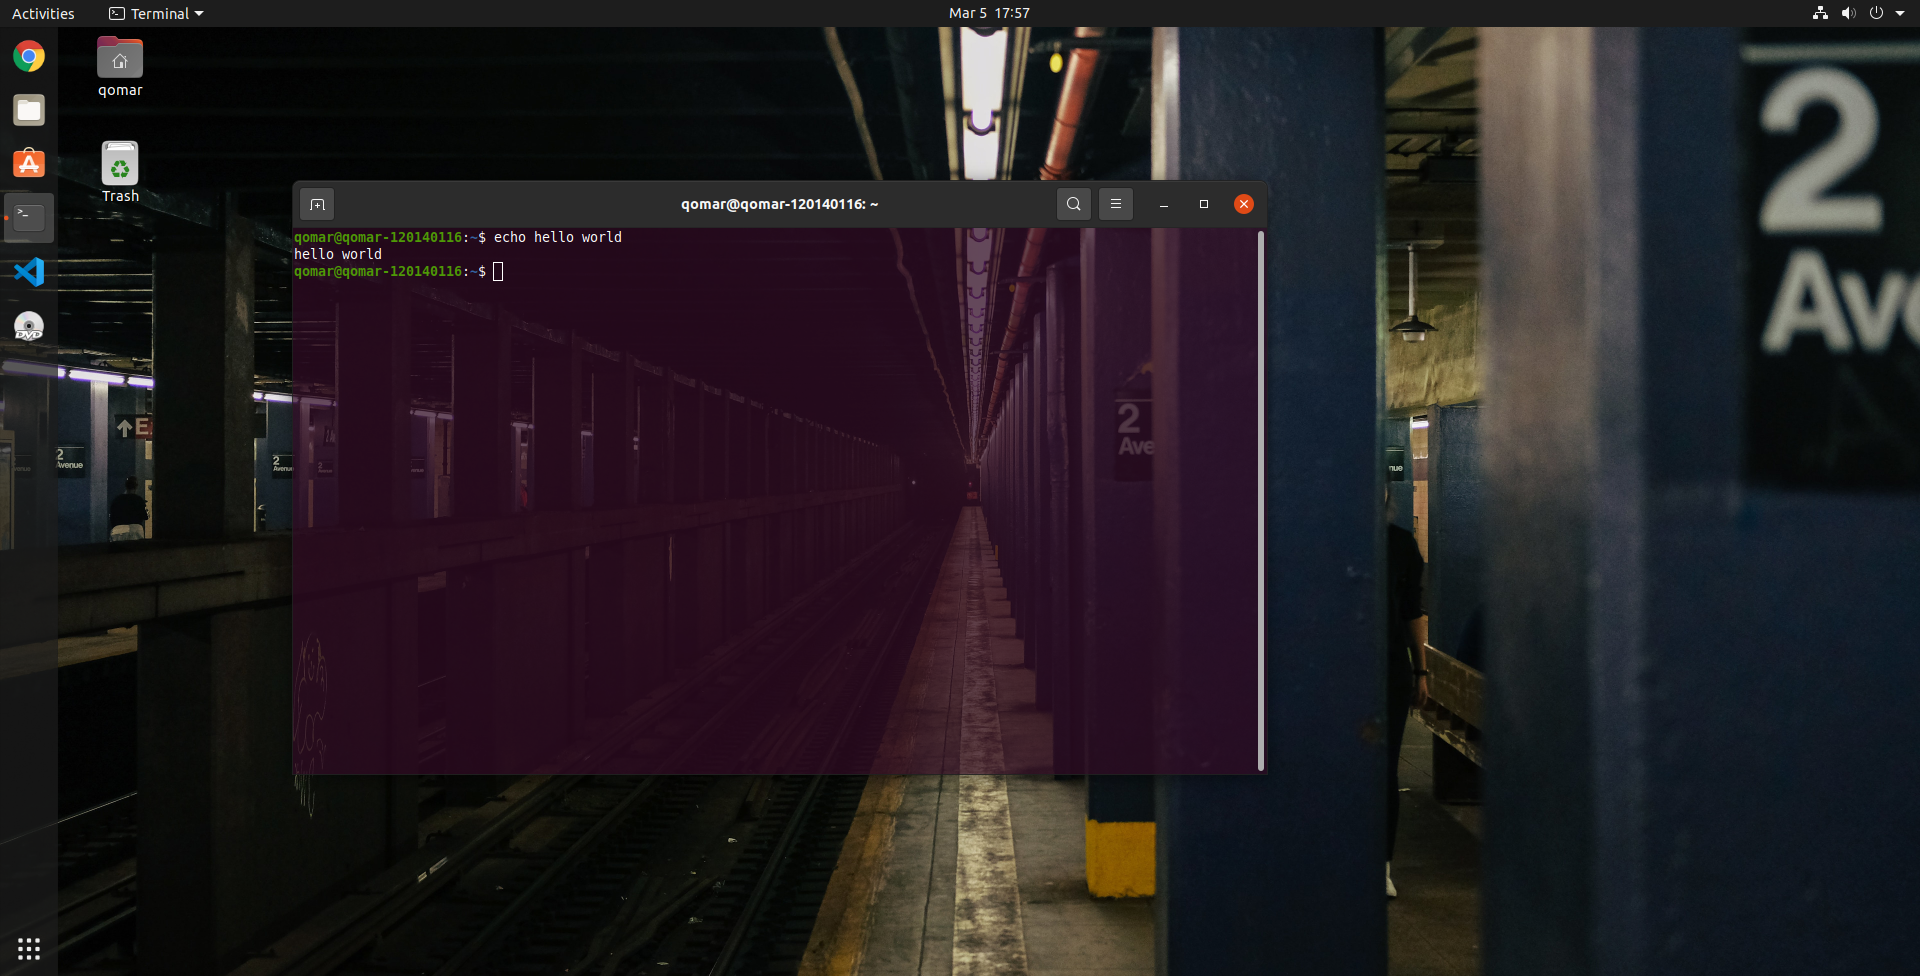
\includegraphics[width=0.8\textwidth]{figure/tut1_bagian1.png}
		\caption{perintah \textit{echo}}
	\end{figure}

\subsection{Tut 1.2 man}
	Pada bagian ini menjalanan perintah sistem yang bermana \textit{man}. \textit{man} merfungsi untuk menjalankan page maunal. Dan menampilkan manual user untuk syntak yang di inputkan setelahnya.
    
	\begin{figure}[h]
		\centering
		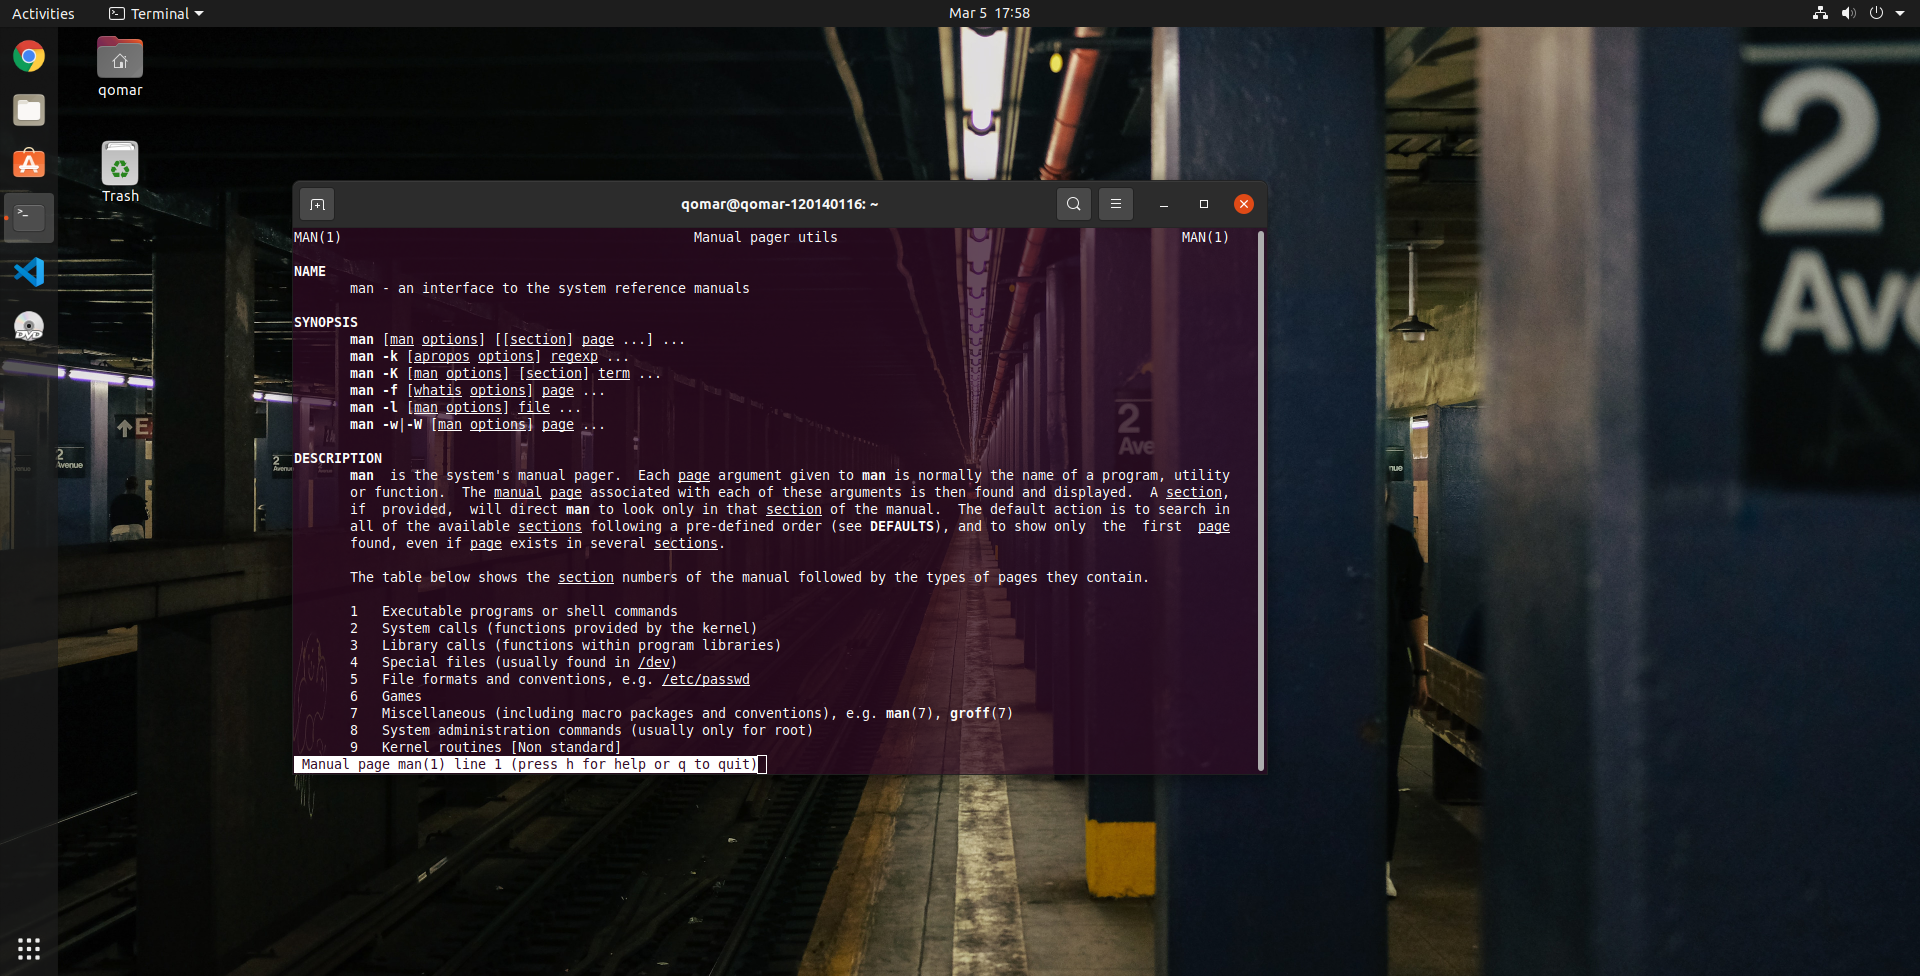
\includegraphics[width=0.8\textwidth]{figure/tut1_bagian2.png}
		\caption{periuntah \textit{man}}
	\end{figure}

\subsection{Tut 1.3 \textit{echo Shell}}
	Pada bagian ini menjalanan perintah sistem yang bermana \textit{echo}, akan tetapi perintah selanjutnya si ketikan \textit{Shell} dan \textit{bin/bash}.
	Maka sitem akan mencetak alamat \textit{bin/bash} dan juga "bin/bash" sebagai kata yang dicetakan.
	\begin{figure}[h]
		\centering
		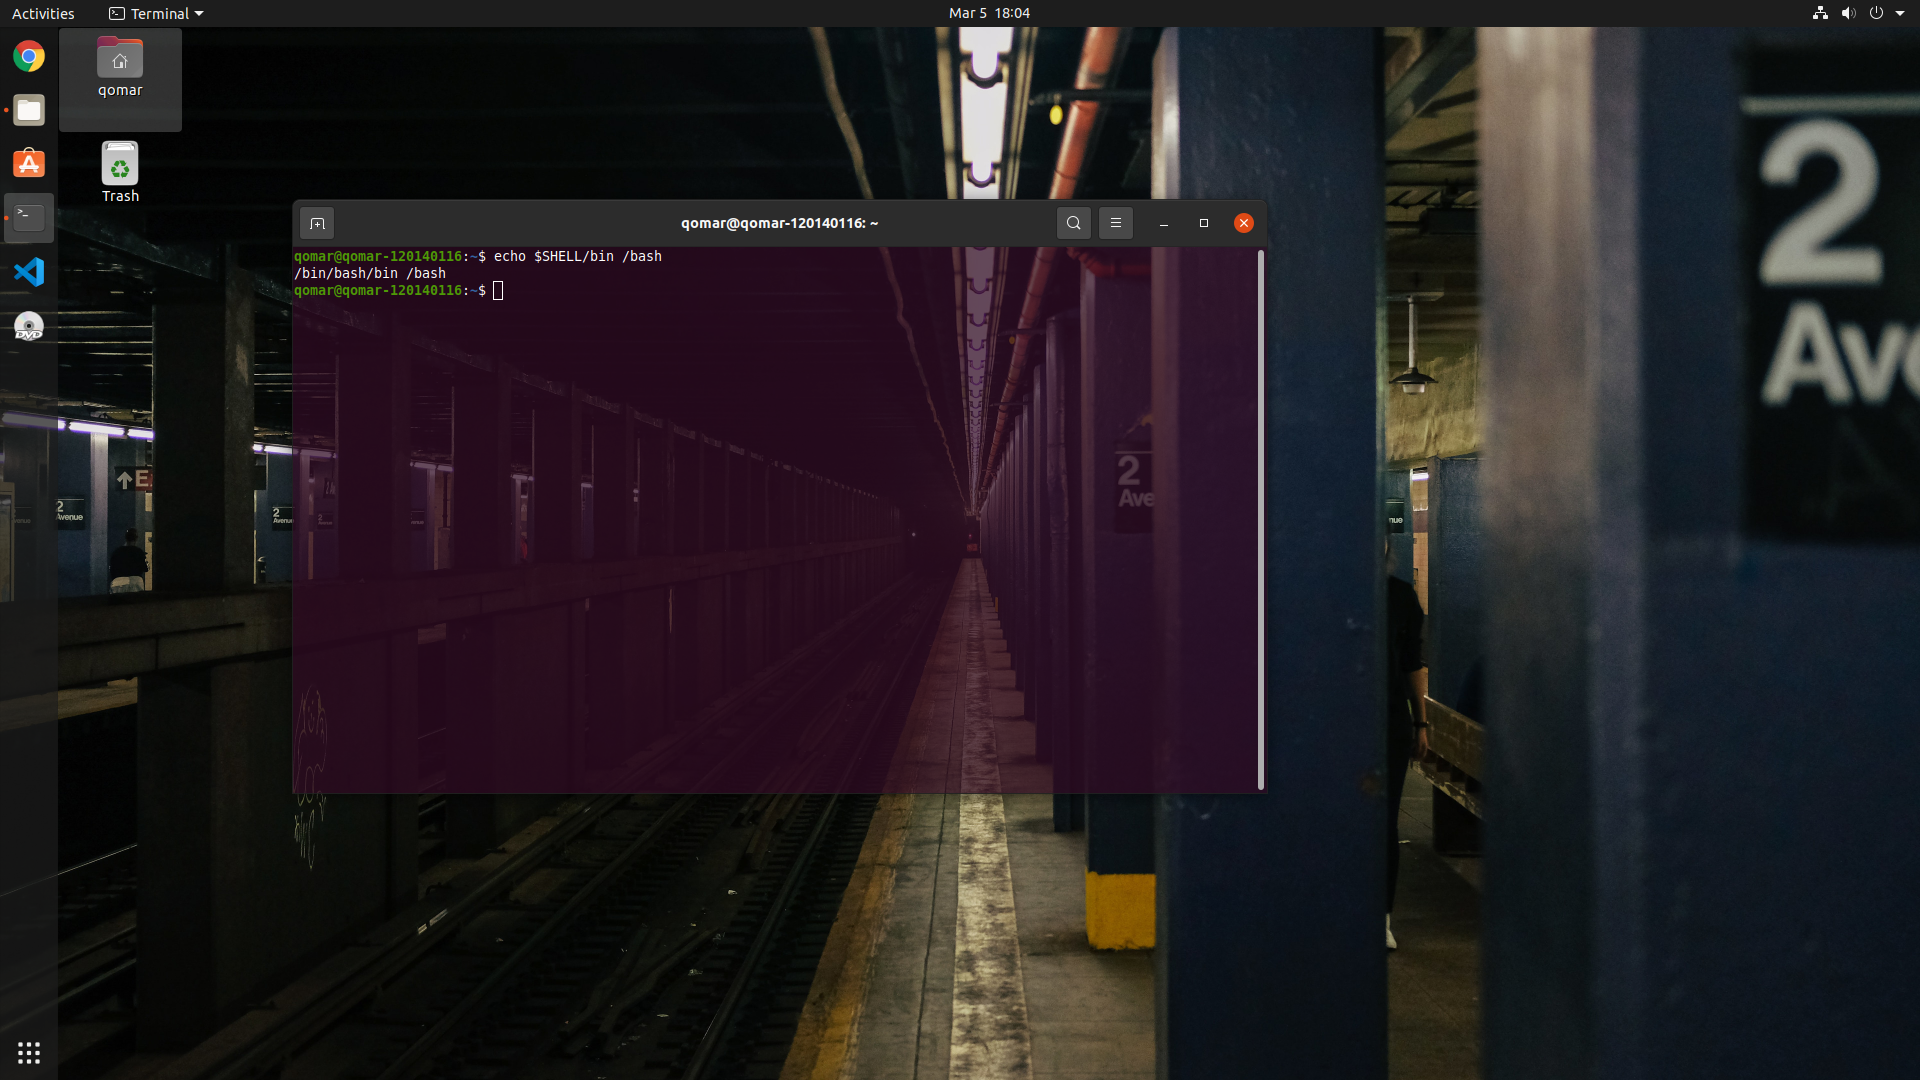
\includegraphics[width=0.8\textwidth]{figure/tut1_bagian3.png}
		\caption{perintah echo Shell}
	\end{figure}

\subsection{Tut 1.4 menjalankan beberapa \textit{comand} linux}
	Pada bagian 4 mahasiswa diminta untuk mempelajari berapa \textit{comand} bash linux melalui page \textit{man} dan kemudian menjalankanya.
	\begin{figure}[h]
		\centering
		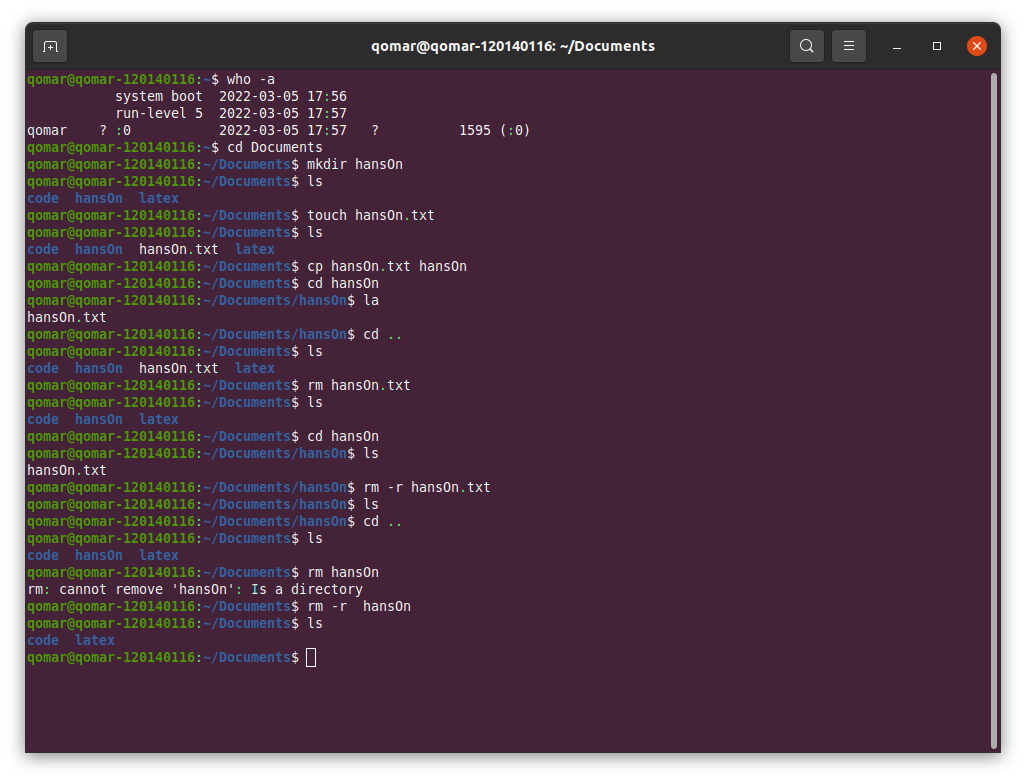
\includegraphics[width=0.6\textwidth, ]{figure/tut1_bagian4.png}
		\caption{menjalankan beberapa \textit{comand} linux}
	\end{figure}


\section{Pembahasan Tut 2}
Pada Tut 2 kita diminta untuk membuat sebuah file yang berjenis txt, yang berisi beberapa baris kalimat. kemudian kita diminta memasukan perintah \textit{sed} untuk menghapus 1 huruf awal dan 1 huruf akhir di setiap baris. selain itu kita juga diminta untuk memasukan \textit{grep} untuk mencari suatu kata dan mengeluarkan berapa kali kata tersebut kelauar.
	\begin{figure}[h]
		\centering
		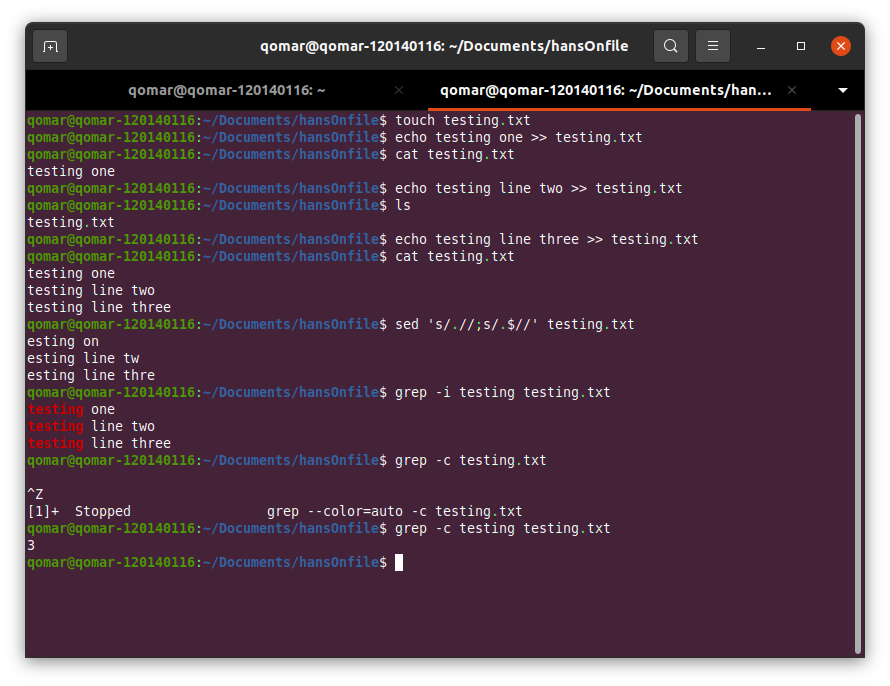
\includegraphics[width=0.8\textwidth]{figure/tut2.png}
		\caption{Perintah \textit{sed} dan \textit{sed}}
	\end{figure}
\subsection*{perintah sed}
	\textit{sed} berfungsi untuk menghapus \textit{string} atau \textit{char} tergantung formating yang diberikan.
	
\subsection*{perintah grep}
	\textit{sed} berfungsi untuk mencari suatu \textit{string} atau \textit{char} yang ada di sebuah file. \textit{sed} juga dapat menentukan berapakali \textit{string} atau \textit{char} tersebut keluar di sebuah file dengan cara menginputkan formating "-c" setelah syntak \textit{sed} 

\newpage
\section{Pembahasan Tut 3}
\begin{figure}[h]
	\centering
	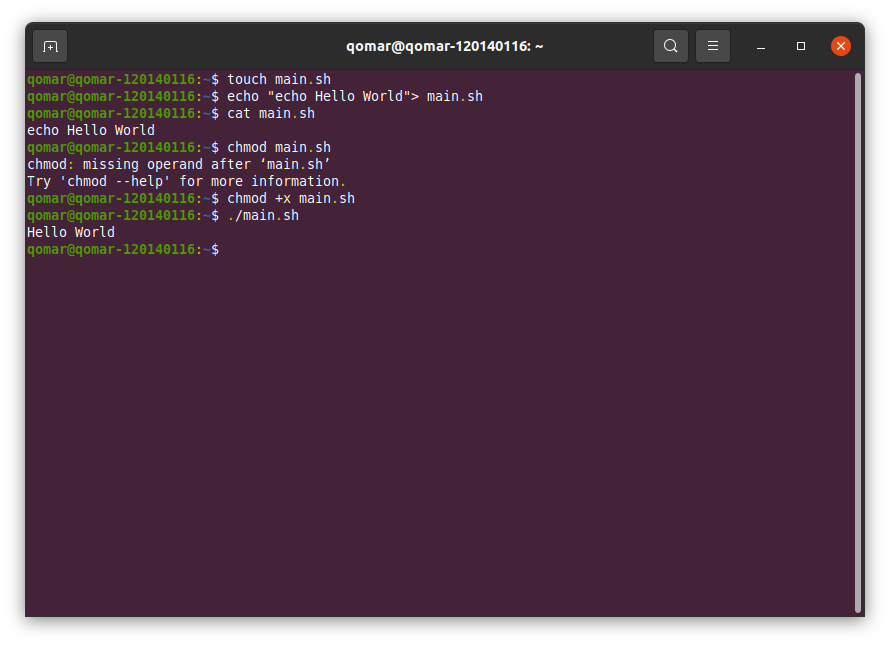
\includegraphics[width=0.8\textwidth ]{figure/tut3.png}
	\caption{Tut 3}
\end{figure}
	Sada bagian Tut 3, user membuat sebuah file baru dengan sh. file ini dapat di buat dengan menegtikan \textit{touch} [nama file]. kemudian file tersebut di isi dengan code \textit{acho Hellwo world}. ini dapat kita lakukan dengan mengetikan \textit{echo "echo hello world" >} [nama File].\\
	Setelah file tersebut jadi, ketikan \textit{cat} [nama file] untuk menampilkan isi penuh dari file tersebut.
	Selanjutnya ketikan \textit{chmod +x } [nama file] dan selanjutnya .$\backslash$ [nama file] untuk menjalankan file tersebut. Maka program akan menampilkan kata yang diketikan tanpa \textit{echo}.

\newpage
\section{Assingment 6}
Pada assingment 6, kita diminta untuk membuat \textit{source code} yang berfungsi untuk mengubah \textit{string} yang ada dalam suatu file yang mulanya terdiri dari huruf kecil ke
huruf bersar semua.
\subsection*{source code}
\begin{lstlisting}[language=bash, caption={source code Assingment 6}]
	# get file name
	echo -n "Enter file name: "
	read file_name
	cat $file_name

	echo " "
	if [ -f $file_name ]
	then
		echo "File exists"
		tr '[a-z]' '[A-Z]' < $file_name
	else
		echo "File does not exist"
	fi

\end{lstlisting}

\subsection*{picture}
\begin{figure}[h]
	\centering
	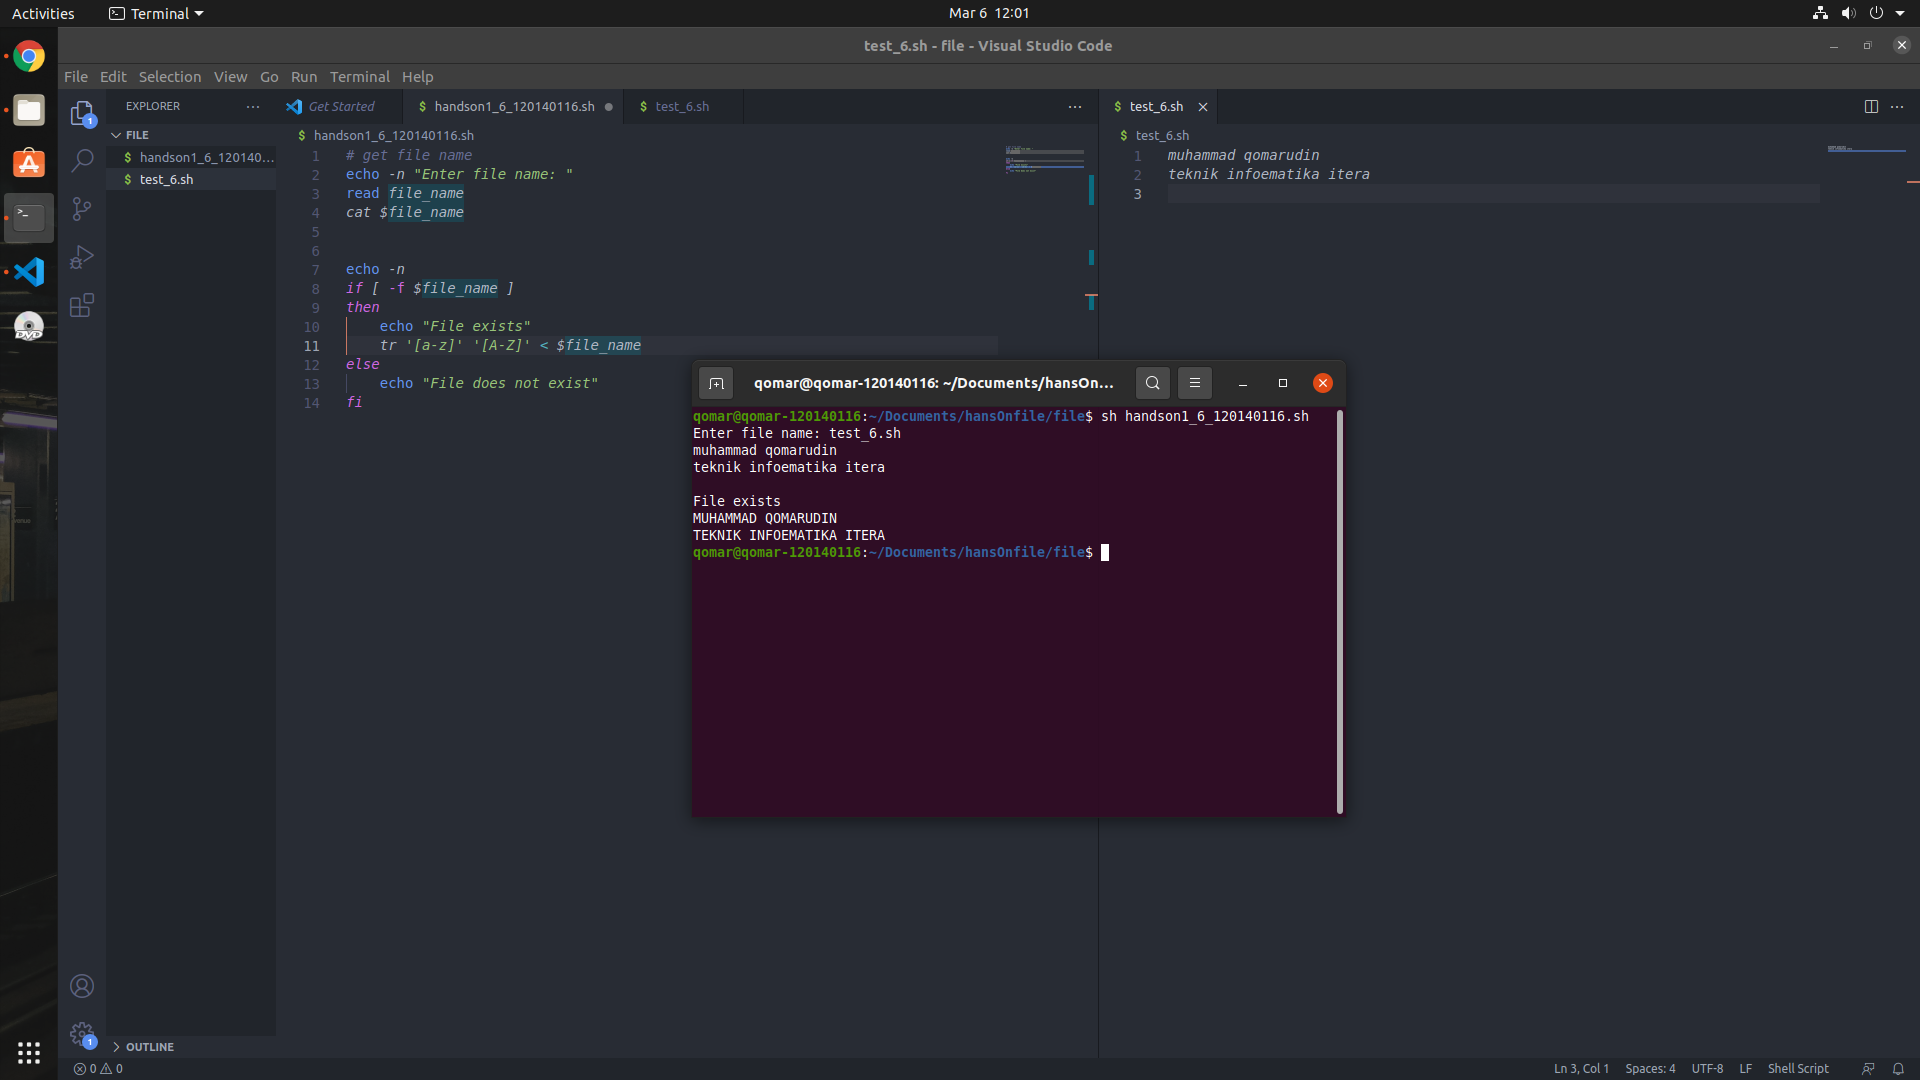
\includegraphics[width=0.93\textwidth]{figure/task_6.png}
	\caption{Detail Assignment 6}
\end{figure}

\newpage
\section{Assingment 8}
perintah assingment 8 adalah memebuat sebuah \textit{code} program yang berfungsi untuk menetukan baris mana yang akan di proses dalam suatu file dengan format .sh atau .txt yang sudah dibuat sebelumnya.
\subsection*{source code}
\begin{lstlisting}[language=bash, caption={source code Assingment 8}]
	echo -n "input file name : "
	read file
	echo -n "input line permulan ynag ingin di outputkan  : "
	read s
	echo -n "input line akhir yang ingin di outputkan  : "
	read n
	sed -n $s,$n\p $file | cat > newline
	cat newline
\end{lstlisting}

\subsection*{picture}
\begin{figure}[h]
	\centering
	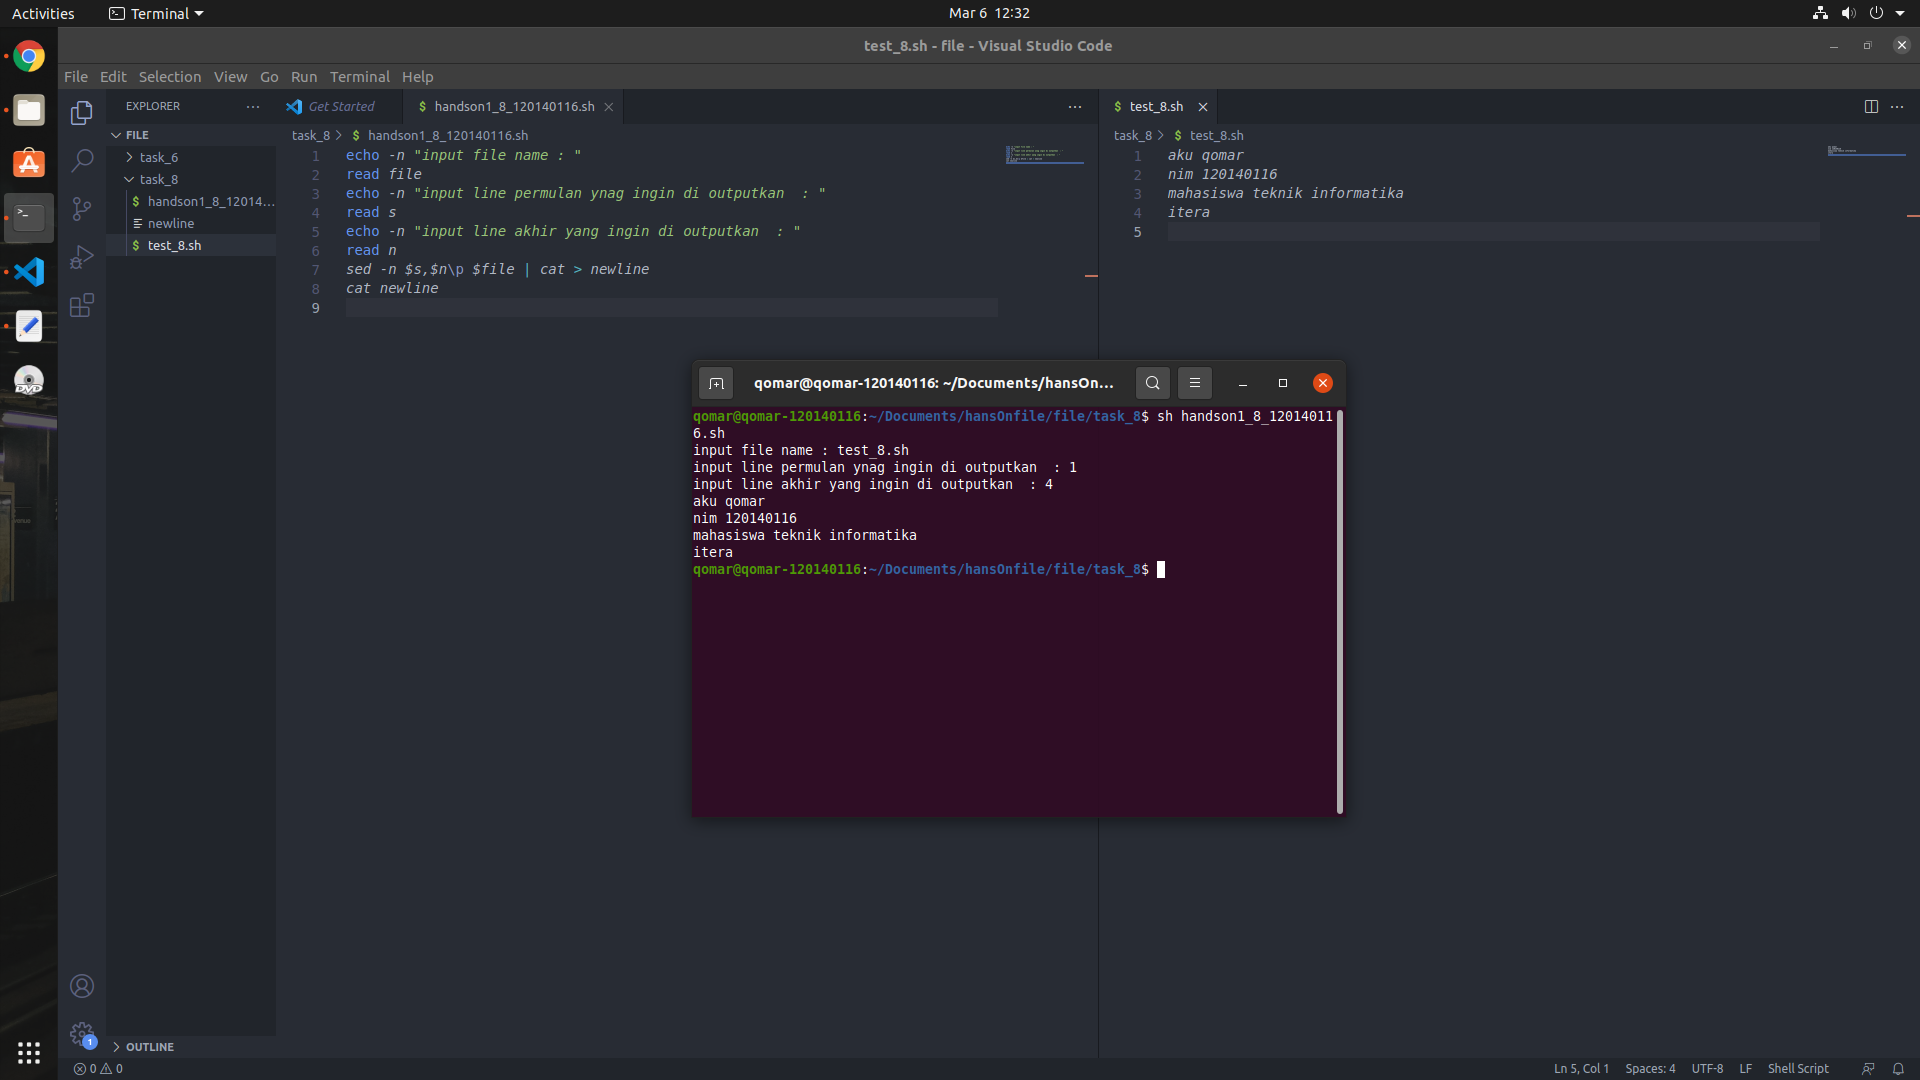
\includegraphics[width=0.93\textwidth]{figure/task_8.png}
	\caption{Detail Assignment 8}
\end{figure}

\newpage
\section{Assingment 9}
Assingment 9 memerintahkan kita unt7k membuat sebuah \textit{code} program yang bertujuan untuk mencari sebuah kata yang ada di dalam suatu file.
Kemudian menghapus \textit{line} dimana kata tersebut berada.
\subsection*{source code}
\begin{lstlisting}[language=bash, caption={source code Assingment 9}]
	echo -n "masukan kata untuk mencocokkan isi dalam line yang akan di hapus : "
	read kata

	for file in $@
	do
		if [ -f $file ]
		then
			echo "ISI SEBELUM DI HAPUS "
			cat $file
			sed -i "/$kata/d" $file

			echo \ "ISI SETELAH DI HAPUS "
			cat $file
		else 
			echo "file tidak ada"
		fi
	done
	echo -n
\end{lstlisting}

\subsection*{picture}
\begin{figure}[h]
	\centering
	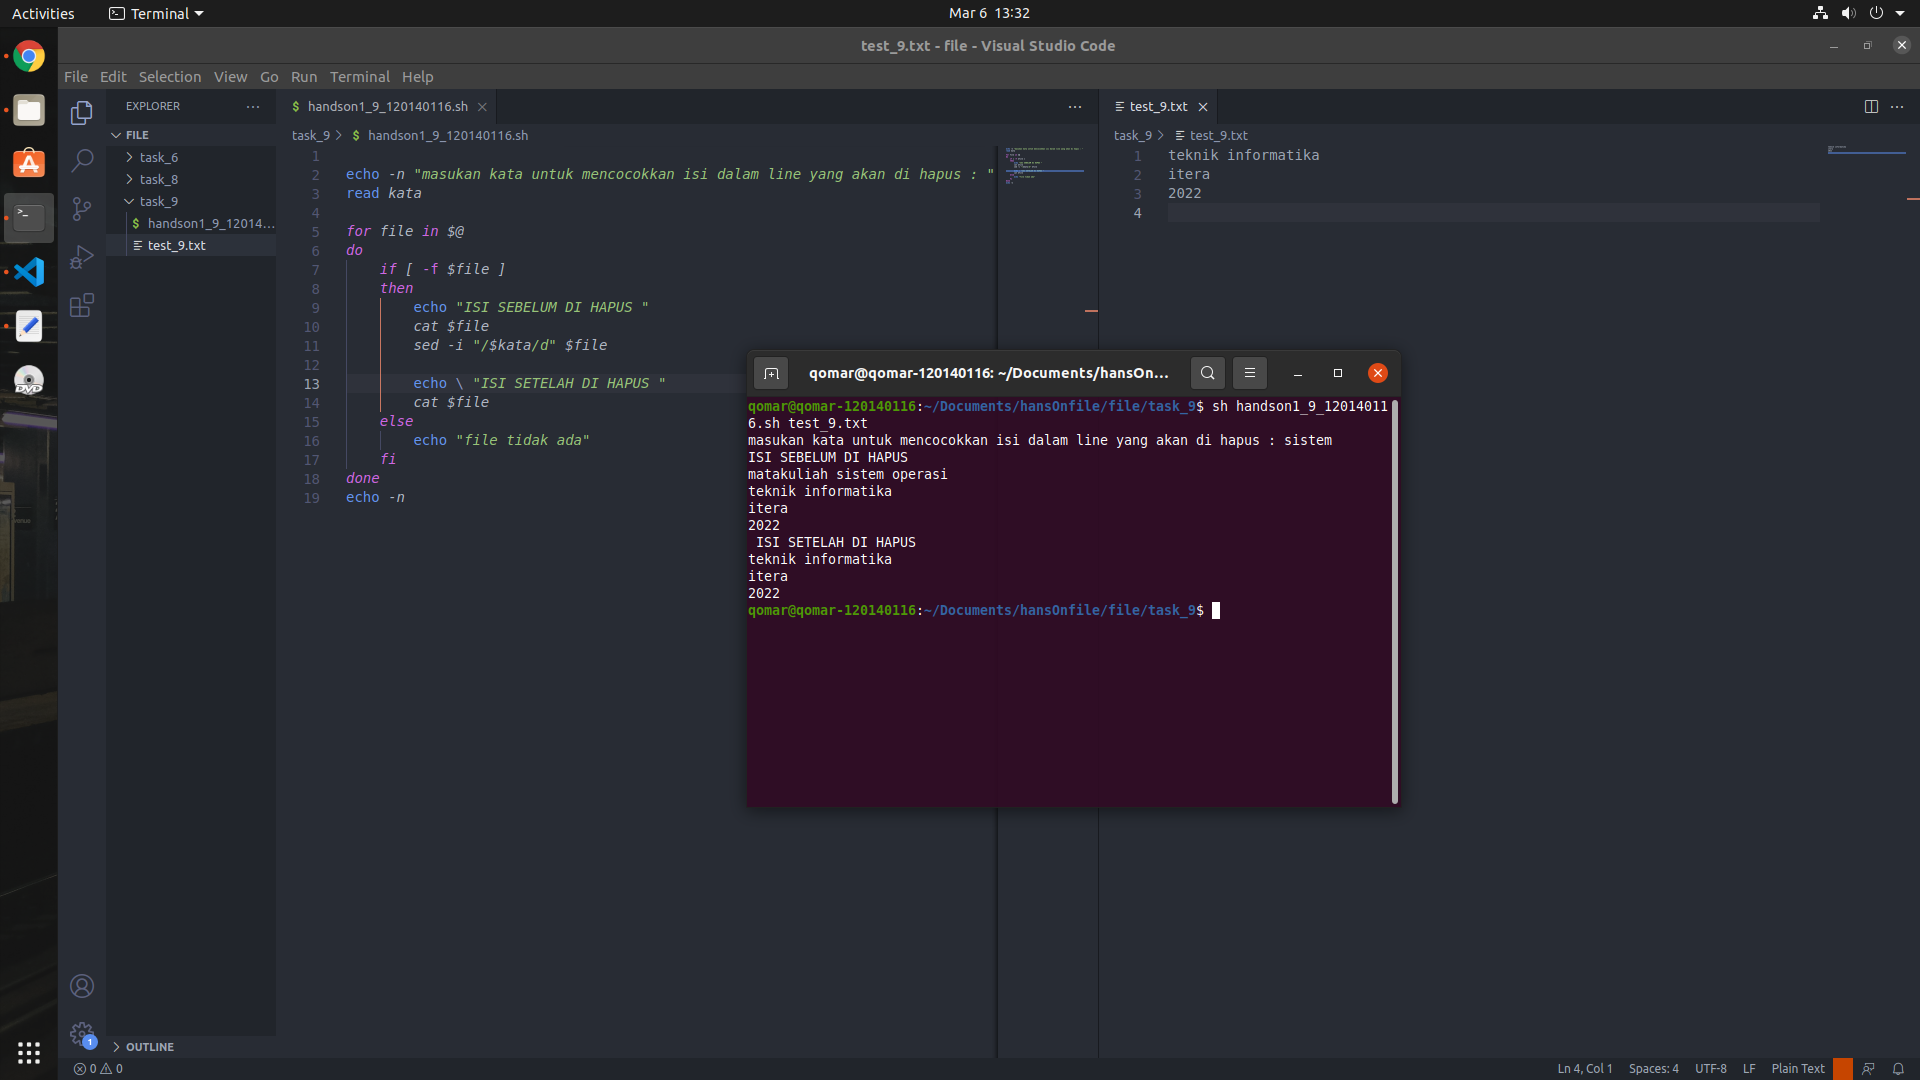
\includegraphics[width=0.93\textwidth]{figure/task_9.png}
	\caption{Detail Assignment 9}
\end{figure}





\newpage
\section{Memuat Gambar}
Berikut ini adalah contoh cara untuk memuat multi-gambar.
\begin{figure}[h]
    \centering
    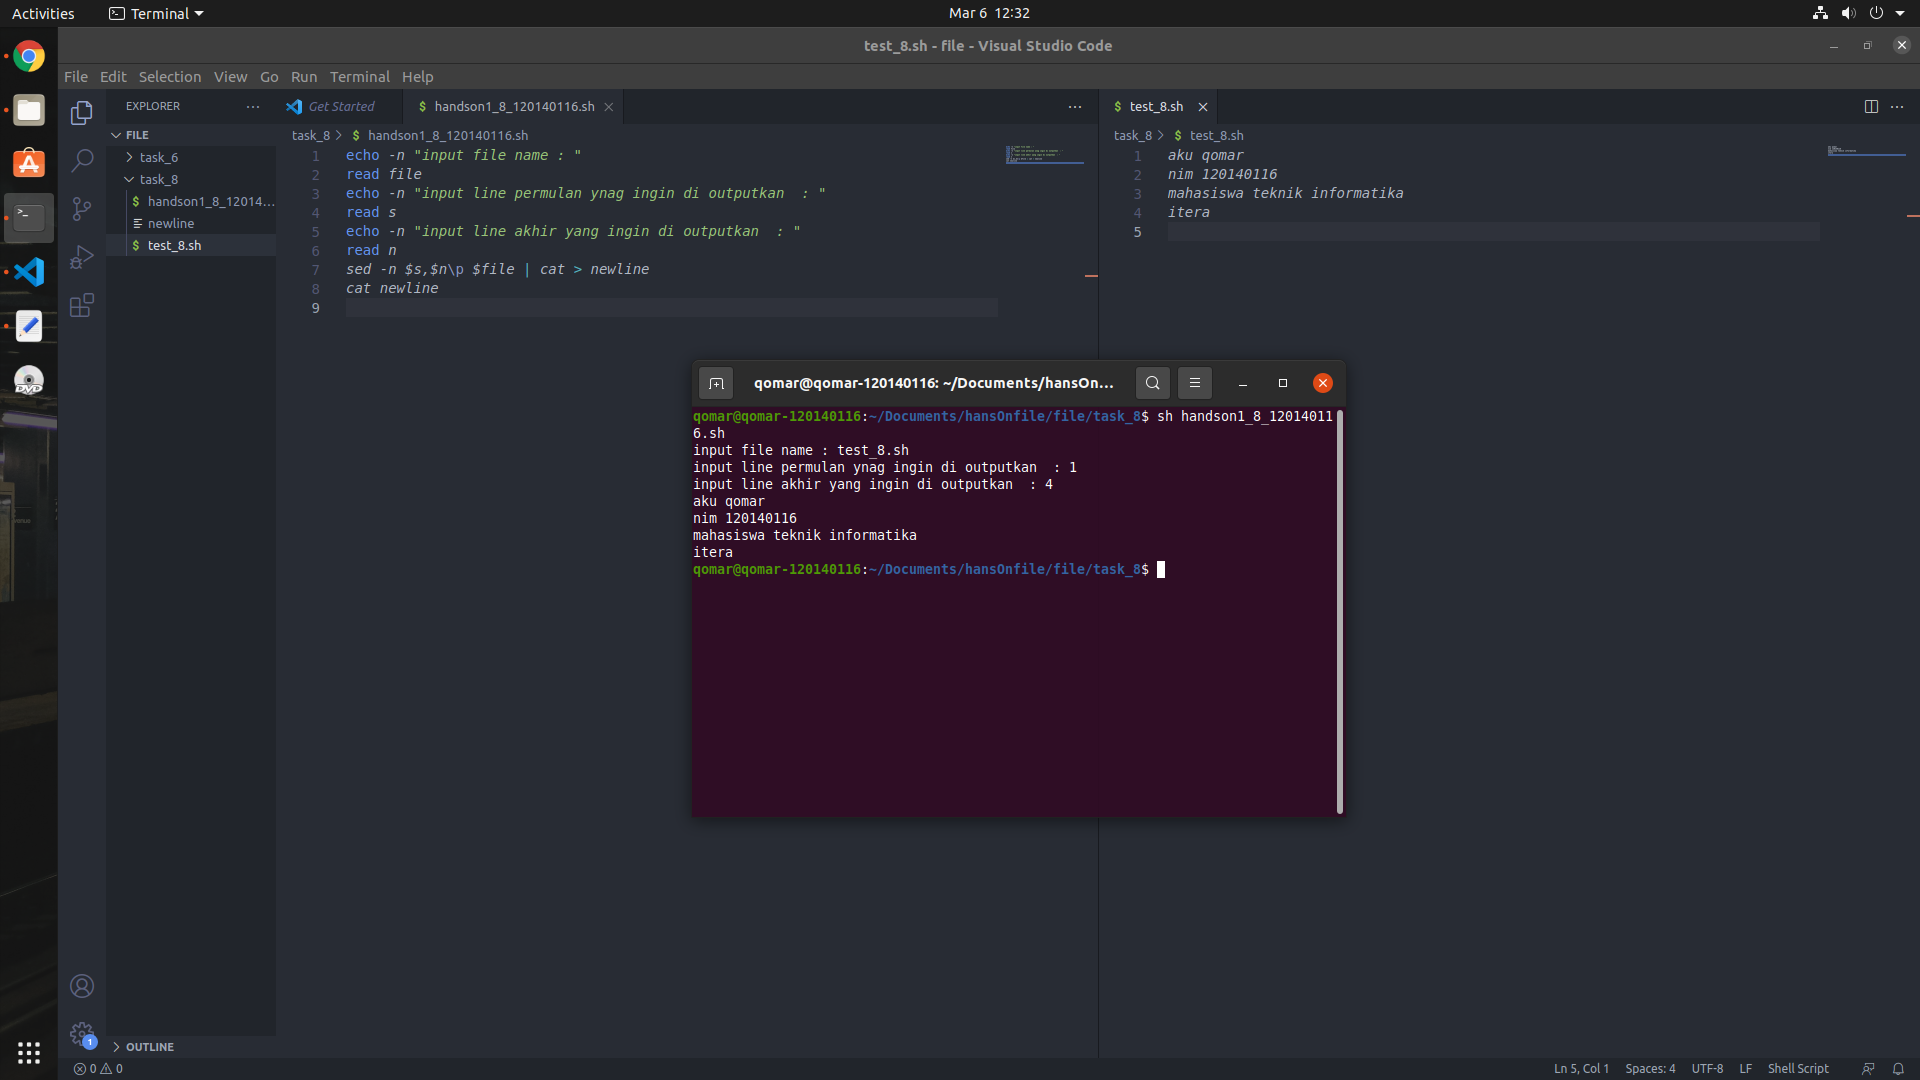
\includegraphics[width=0.93\textwidth]{figure/task_8.png}
    \caption{Ini Captionnya}
    \label{fig:my_label}
\end{figure}

\newpage
\bibliographystyle{IEEEtran}
\bibliography{Referensi}
\end{document}